\documentclass[draft=false
              ,paper=a4
              ,twoside=false
              ,fontsize=11pt
              ,headsepline
              ,BCOR10mm
              ,DIV11
              ]{scrbook}
\usepackage[ngerman,english]{babel}
%% see http://www.tex.ac.uk/cgi-bin/texfaq2html?label=uselmfonts
\usepackage[T1]{fontenc}
%\usepackage[utf8]{inputenc}
\usepackage[latin1]{inputenc}
%\usepackage[macce]{inputenc}
\usepackage{libertine}
\usepackage{pifont}
\usepackage{microtype}
\usepackage{textcomp}
\usepackage[german,refpage]{nomencl}
\usepackage{setspace}
\usepackage{makeidx}
\usepackage{listings}
\usepackage{natbib}
\usepackage[ngerman,colorlinks=true]{hyperref}
\usepackage{soul}
\usepackage{hawstyle}
\usepackage{lipsum} %% for sample text


%% define some colors
\colorlet{BackgroundColor}{gray!20}
\colorlet{KeywordColor}{blue}
\colorlet{CommentColor}{black!60}
%% for tables
\colorlet{HeadColor}{gray!60}
\colorlet{Color1}{blue!10}
\colorlet{Color2}{white}

%% configure colors
\HAWifprinter{
  \colorlet{BackgroundColor}{gray!20}
  \colorlet{KeywordColor}{black}
  \colorlet{CommentColor}{gray}
  % for tables
  \colorlet{HeadColor}{gray!60}
  \colorlet{Color1}{gray!40}
  \colorlet{Color2}{white}
}{}
\lstset{%
  numbers=left,
  numberstyle=\tiny,
  stepnumber=1,
  numbersep=5pt,
  basicstyle=\ttfamily\small,
  keywordstyle=\color{KeywordColor}\bfseries,
  identifierstyle=\color{black},
  commentstyle=\color{CommentColor},
  backgroundcolor=\color{BackgroundColor},
  captionpos=b,
  fontadjust=true
}
\lstset{escapeinside={(*@}{@*)}, % used to enter latex code inside listings
        morekeywords={uint32_t, int32_t}
}
\ifpdfoutput{
  \hypersetup{bookmarksopen=false,bookmarksnumbered,linktocpage}
}{}

%% more fancy C++
\DeclareRobustCommand{\cxx}{C\raisebox{0.25ex}{{\scriptsize +\kern-0.25ex +}}}

\clubpenalty=10000
\widowpenalty=10000
\displaywidowpenalty=10000

% unknown hyphenations
\hyphenation{
}

%% recalculate text area
\typearea[current]{last}

\makeindex
\makenomenclature

\begin{document}
\selectlanguage{ngerman}


%%%%%
%% customize (see readme.pdf for supported values)
\HAWThesisProperties{Author={Jan Lepel}
                    ,Title={Automatisierte Erstellung und Provisionierung von ad hoc Linuxumgebungen -\\  Prototyp einer zentralisierten Weboberfl�che zur vereinfachten Umsetzung individuell erstellter Systeme}
                    ,EnglishTitle={TODO}
                    ,ThesisType={Bachelorarbeit}
                    ,ExaminationType={Bachelorpr�fung}
                    ,DegreeProgramme={Bachelor of Science Angewandte Informatik}
                    ,ThesisExperts={Prof. Dr. Ulrike Steffens \and MSc Informatik Oliver Neumann}
                    ,ReleaseDate={1. Januar 2015}
                  }

%% title
\frontmatter

%% output title page
\maketitle

\onehalfspacing

%% add abstract pages
%% note: this is one command on multiple lines
\HAWAbstractPage
%% German abstract
{Ad hoc Umgebung, automatisierter Umgebungsaufbau und Provisionierung}%
{Dieses Dokument \ldots}
%% English abstract
{Keywords, Keywords1}%
{This document \ldots}

\lstlistoflistings

%% main


\newpage
\singlespacing

\tableofcontents
\newpage
%% enable if these lists should be shown on their own page
%%\listoftables
%%\listoffigures

%%\lstlistoflistings

%% main
\mainmatter
\onehalfspacing
%% write to the log/stdout
\typeout{===== File: chapter 1}
%% include chapter file (chapter1.tex)
%%\include{chapter1}

\chapter{Einleitung}
\begin{quote}
	``Es ist nicht zu wenig Zeit, die wir haben, sondern es ist zu viel Zeit, die wir nicht nutzen'' - Lucius Annaeus Seneca, \cite{Apelt200511}
\end{quote}
Seneca formulierte  49 n. Chr. ein Gef"uhl das jeder kennt. Die Zeit die er hat, nicht richtig zu nutzen.
Technische Neuerungen helfen uns unsere Zeit besser zu planen, mehr Zeit in andere Aktivit�ten zu stecken und unsere Priorit�ten zu "uberdenken.
Diese Arbeit besch�ftigt sich mit dem Teil-Aspekt der Informatik, der Virtualisierung von Servern im Entwicklungsumfeld.\newline
... 



\section{Motivation}

\section{Zielsetzung}
Das Ziel der vorliegenden Arbeit ist es, durch inkrementelles und interatives Vorgehen eine Applikation zu modellieren, die den Anwender der Applikation bei dem Aufbau von virtuellen Umgebungen unterst�tzt. Je nach Wunsch des Anwenders, wird nicht nur der Aufbau einer Umgebung vereinfacht, sondern auch die direkte Installation von Programmen veranlasst. Eine Weboberfl�che soll die entsprechenden Optionen zur Verf�gung stellen und dem Anwender durch seine ausgew�hlte Funktion leiten.
Gro�e Konfigurationen oder komplizierte Einstellungen sollen dem Normalanwender abgenommen werden und geschehen im Hintergrund. 
Damit auch ein Sichern oder ein Zur�ckspielen von vorhandenen virtuellen Maschinen m�glich wird, sollten Im- und Exportfunktionen dies untzerst�tzen.
Die Realisierung sollte auf einem zentralen Knotenpunkt stattfinden, um es mehreren Anwendern zu erm�glichen, ihre notwendige Maschine zu erstellen und zu verwalten.
Kernaufgaben sollen Open-Source Anwendungen �bernehmen, die in ihrem Bereich etabliert sind. Ebenfalls im Fokus steht die Leichtigkeit der Konfiguration der auszuw�hlenden Open-Source Anwendung.
Bei der Erstellung der einzelnen Softwarekomponenten ist stehts auf das Prinzip von hoher Koh�sion und loser Kopplung zu achten. Also dem Grad der Abh�ngigkeit zwischen mehrere Hard-/ und Softwarekomponenten, der �nderungen an einzelnen Komponenten erleichtert.
Um auch die Anwendungsoberfl�che unkompliziert zu halten, soll der Anwender mit ein paar Klicks zu seinem Ziel gef�hrt werden. Durch das Vermeiden von unn�tigen Verschachtelungen oder einer Flut an Optionen und Konfigurationen, soll der Anwender in der Applikation einen Helfer f�r seine T�tigkeit finden.
\newline


\begin{comment}
\section{Zielsetzung}
Ziel der vorliegenden Arbeit ist es, ein Softwareprodukt zu erarbeiten, welches aktuelle Virtualisierungs-, sowie Provisionierungsl�sungen verwendet, um mit deren Hilfe den Aufbau von tempor�ren (ad hoc) Umgebungen im virtuellen Umfeld zu vereinfachen.\newline
Eine Auswahl von leicht erlernbaren und unkomplizierten Softwarekomponenten, f�rdern ein weiteres Ziel. Den Administrationsaufwand gering wie m�glich zu halten und auch Linux/Unix unerfahrene Administratoren, sowie Entwickler anzusprechen.\newline
Es ist angestrebt, bei Ende dieser Arbeit eine zentralisierte und leicht lokal zu implementierende Anwendung zur Verf�gung zu stellen.
Sie soll es dem Benutzer erm�glichen, sich selbstst�ndig und mit geringem Zeitaufwand eine virtuelle Maschine mit gew�nschter Software zu erstellen, ohne gro�e Einarbeitung in Benutzung und Konfiguration. \newline
Somit wird die administrative Instanz des z.B. Unternehmen entlasten und bef�higt den Benutzer sich auf seine Kernt�tigkeiten zu konzentrieren.



\section{Problemstellung}
%Die Einleitung muss Ihr Thema eingrenzen (und diese Eingrenzung rechtfertigen) und Ihr Erkenntnisinteresse präzisieren und begründen
Virtualisierung hat in vielen Bereichen den physischen Server abgel�st, denn der Finanzielle Aspekt ist f"ur Unternehmen nicht unerheblich. Im Idealfall hei�t der Umstieg auf virtuelle Landschaften gleich weniger Server, was gleichbedeutend mit weniger Stellfl�che ist. Somit auch mit weniger Racks und weniger Verkabelung.\newline
Aufw�ndige Vorplanung von Serverzentren entf�llt, die Kostenplanung der unterschiedlichen Hardware wird minimiert und die Frage, was in ein paar Jahren mit der Hardware passieren soll, wird obsolet.\newline
Gerade im Entwicklungsbereich ist es meist sinnvoller virtuelle Umgebungen zu realisieren, als reale Maschinen aufzubauen. Entwickler haben so die M�glichkeit bei Bedarf sich Abz"uge der Produktionsumgebung zu erstellen oder Fehlerszenarien nachzustellen.\newline
Meist ist dazu die Involvierung des Betriebs-Teams oder des IT-Support notwendig, die nach Priorit�t ihrer Auftragslage, eine gewissen Vorlaufzeit ben�tigen, um die gew�nschte Maschine aufzubauen. \newline
In dem Fall, dass die Firmengr��e es nicht erlaubt, eine eigene Support-Abteilung zu haben, muss die Zeit des jeweiligen Mitarbeiters herhalten, um das Wissen �ber die jeweilige Virtualisierungsl�sung aufzubauen, die gew�nschte Maschine zu erstellen und die Installationen der n�tigen Programme zu realisieren. Der R�ckschluss daraus ist, geringere Produktivit�t in den Kernt�tigkeiten des Mitarbeiters.\newline
Auch wenn die Softwarebranche eine Vielfalt an M�glichkeiten bereitstellt, sind diese entweder in ihrer Struktur �berdimensioniert, um sie in der Anwendung schnell zu erlernen, oder komplex in ihrer Konfiguration in Bezug auf Automatisierungen und/oder Provisionierungen.

%Da die Softwarebranche vielf�ltige M�glichkeiten bereitstellt, um mit geringem Aufwand lokal eine virtuelle Umgebung zu erzeugen und diese ggf. zu Provisionieren. 
%Im idealfall heisst das f�r Unternehmen: Weniger Server sind gleichbedeutend mit weniger Stellf�che, mit weniger Verkabelung oder Racks. Somit ist die %Konsolidierung der ehemals gro�en Server-Zentren f�r viele Unternehmen eine direkte Konsequenz. 
%Wodurch eine Kostenreduzierung der gesamten Infrastruktur entsteht.\newline
%Nicht nur der Finanzielle Aspekt spricht oft f�r die Virtualisierung, sondern auch die leichte Automatisierung, die Erh�hung der Verf�gbarkeit und ....\newline
%Das Verschieben von kompletten Applikationen von einem physischen Ort zu einem anderen,....\newline
%Verbesserung der Verf�gbarkeit und Business Continuity. Dazu geh�ren Live Migration, Storage Migration, Fehlertoleranz, Hochverf�gbarkeit und Ressourcen-Management. Virtuelle Maschinen k�nnen damit leicht verschoben und vor ungew�nschten Auszeiten gesch�tzt werden.\newline
%In der physischen Welt war es bisher �blich, jeder Applikation einen eigenen Server zuzuweisen. Damit war daf�r Sorge getragen, dass die einzelnen Software-Programme sauber voneinander isoliert waren. Aber das f�hrte auch zu einem Wust von Rechnern, von denen viele noch dazu nicht optimal ausgelastet waren. Und die Kosten f�r diese Server-Landschaft liefen schnell aus dem Ruder. Nicht so bei Virtualisierung. Inzwischen sind auch die n�tigen Funktionen und Tools vorhanden, um VMs und die in ihnen verpackten Anwendungen sauber voneinander zu trennen. CPU, Memory und Storage k�nnen exakt ausgelastet werden, die Kosten in einem solchen Modell sinken.\newline



\section{Motivation}
Die Motivation dieser Ausarbeitung besteht darin, eine Software zu entwickeln, die durch vereinfachte Handhabung und minimaler Einarbeitungszeit, es dem Benutzer erm�glich eine ad-hoc Umgebung zu erstellen, ohne b�rokratischen Aufwand und ohne Grundwissen �ber die darunterliegende Anwendungsstruktur.
Der normalerweise gro�e zeitliche Aufwand soll m�glichst minimiert werden und es Anwendern in Unternehmen und Projekten erleichtert wird, sich auf die vorhandenen Usecase zu fokussieren und keine Zeit in Aufbau, Installation und Problembehebung investieren zu m�ssen.

\section{Themenabgrenzung}
Diese Arbeit greift bekannte und etablierte Softwareprodukte auf und nutzt diese in einem zusammenh�ngenden Kontext. Dabei werden die verwendeten Softwareprodukte nicht modifiziert, sondern f�r eine vereinfachte Benutzung durch eigene Implementierungen kombiniert und mit einem Benutzerinterface versehen, welches die Abl�ufe visualisiert und dem Benutzer die Handhabung vereinfacht.
Die vorzunehmenden Implementierungen greifen nicht in den Ablauf der jeweiligen Software ein, sondern vereinfacht das Zusammenspiel der einzelnen Anwendungen.

\section{Struktur der Arbeit}

\chapter{Grundlagen}
\section{Begriffserkl�rung}
Im Verlauf dieser Arbeit werden Begrifflichkeiten verwendet, die im Vorfeld zu kl�ren sind.\newline
	\begin{enumerate}
		\item \textbf{Provisioning / Provisioner}\newline
\textit{Provisioning} ist ein Aspekt der Informatik, in dem es darum geht, den richtigen Personen zur richtigen Zeit effektiv Ressourcen zur Verf�gung zu stellen.
\textit{Provisioner} helfen bei der Softwareverteilung auf gew�nschte Maschinen, Ad-hoc Kommando-Ausf�hrung und Konfigurationsmanagement.
In dieser Arbeit bezieht sich der Begriff \textit{Provisioning} auf die automatisierte Softwareverteilung, die mit dem Aufbau einer Entwicklungsumgebung verbunden ist.\newline
		\item \textbf{Entwicklungsumgebung}\newline
IDE's (integrated development environment) sind Entwicklungsumgebungen, die den Entwickler unterst�tzen, Quellcode zu schreiben und zu bearbeiten. Die g�ngigsten IDE's unterst�tzen mei�t mehrere Programmiersprachen und helfen dem Entwickler mit n�tzlichen Funktionen, wie  z.B. das aufzeigen von Fehlern im Quelltext. Entwicklungsumgebungen sind in vielen F�llen auch PC's / Server / virtuelle Maschinen, die zum Entwickeln installiert und bereitgestellt werden.
Dort k�nnen neue Funktionalit�ten ausprobiert werden und das bestehende System testweise erweitert werden, ohne in die Produktionslandschaft einzugreifen.
In den folgenden Texten wird der Begriff \textit{Entwicklungsumgebung} als Synonym f�r eine virtuelle Maschine benutzt, die dem Anwender die Freiheit gibt, unkompliziert M�glichkeiten auszutesten und neues auzuprobieren.\newline
		\item \textbf{Aufbau einer Maschine}\newline
\textit{Aufbau einer Maschine} beinhaltet immer das automatische Erstellen und Konfigurieren einer virtuellem Maschine mit Hilfe von VirtualBox und Vagrant.
Das Resultat ist eine virtuelle Maschine mit der Basisinstallation von Ubuntu (32Bit / 64Bit) und \textbf{MEHR INFOS ZU DEM SYSTEM}.
Durch die M�glichkeit des Provisioning kann die Basisinstallation mit Software erg�nzt und Befehle auf der Maschine ausgef�hrt werden.

\item \textbf{Maschinenkonfiguration}\newline
F�r den Aufbau einer Maschine werden zwei wesentliche Konfigurationsdateien erstellt.
Diese werden f�r den Aufbau der virtuelle Maschine selbst ben�tigt und f�r das ggf. gew�nschte Provisioning. Der Begriff \textit{Maschinenkonfiguration} beschreibt im folgenden immer das vorhandensein beider Dateien. 
	\end{enumerate}
	

\end{comment}
\chapter{Anforderungen}
An dieser Stellen sollen die Anforderungen an die Software detaillierter konzipiert und aufgelistet werden.\newline
Ein direkter Vergleich mit bestehenden L�sungen wird veranschaulicht und das Konzept der zu entwickelnden Software genauer betrachtet.

\section{Funktionale Anforderungen}
Funktionale Anforderungen beschreiben Dienste oder Funktionalit�ten, die ein System bereitstellen soll.\newline
  \begin{enumerate}
      \item[FA 1.0] \textbf{Berechtigungssystem}\newline
		Die zu entwickelnde Software soll zwei Berechtigungsstufen beinhalten, um Benutzer und Administratoren von einander zu trennen.
		\begin{enumerate}      
		    \item[FA 1.1] Rolle: Administrator\newline
                                  Die Administrator-Rolle, soll Zugriff auf konfigurative M�glichkeiten bekommen.\newline 
							   Beispiele hierf�r w�ren: Speicherpfad der Logdatei �ndern; neue Softwarekomponenten in die Auswahlliste(FA 2.0) �bernehmen.
			\item[FA 1.2] Rolle: User\newline
							   Benutzer in der User-Rolle sind nicht berechtigt Konfigurationen an der Software vorzunehmen. Ihnen steht der Administrative Punkt nicht zur
							    Verf�gung
		\end{enumerate}      
   \end{enumerate}        
      
  \begin{enumerate}
      \item[FA 2.0] \textbf{Ausswahlliste Softwarekomponenten}\newline
       Um dem Benutzer die M�glichkeit zu bieten, auf die gew�nschte Maschine Softwarekomponenten zu provisionieren, soll das System eine entsprechende 				   Auswahlliste beinhalten
		\begin{enumerate}      
		    \item[FA 2.1] Die Auswahlliste kann durch Benutzer mit Administrationsberechtigungen ge�ndert werden. Benutzer mit Berechtigungen der Stufe 									   \textbf{User}, d�rfen die Liste nicht manipulieren.\newline
			\item[FA 2.2] Folgende Funktionen sollen dem Administrator zur Verf�gung gestellt werden:
			\begin{enumerate}      
						\item L�schen - L�scht den kompletten Datensatz aus der Liste und somit aus der Datenbank.
						\item �ndern - Beschreibung, sowie Linux-Befehlssatz kann ge�ndert werden.
						\item Hinzuf�gen - Name der Software, Beschreibung und Linux-Befehlssatz k�nnen eingegeben werden und zur Datenbank hinzugef�gt werden.
		    \end{enumerate}      
		\end{enumerate}      
   \end{enumerate}        
      
  \begin{enumerate}
      \item[FA 3.0] \textbf{Hochladen eigener YAML-Dateien}\newline
		Es soll m�glich sein, statt die Auswahlliste(FA 2.0) zu verwenden, eine YAML-Datei hochzuladen, die die gew�nschte Software enth�lt.\newline
		Dies geschieht �ber einen Men�punkt in der Benutzeroberfl�che.
		\begin{enumerate}      
		    \item[FA 3.1] Die YAML-Datei muss den Vorgaben von Ansible gen�gen.
		    \item[FA 3.2] Administratoren und User d�rfen YAML-Dateien verwenden.
			\item[FA 3.3] Fehler sind in einer Logdatei zu protokolieren.
		\end{enumerate}      
   \end{enumerate}        
   
  \begin{enumerate}
      \item[FA 4.0] \textbf{Fehler}\newline
	  Falsche Benutzung oder Systemfehler sollen Software angezeigt werden und entsprechend in einer Logdatei protokoliert werden.
		\begin{enumerate}      	  
		  \item[FA 4.1] Falsche Benutzung, darf nicht zum Abbruch des kompletten Vorgangs f�hren.
		\end{enumerate}      
   \end{enumerate}        

%Diese Beschreibung kann in allgemeiner Form Funktionen des Systems definieren oder als Spezifikation detaillierte Aussagen zum gew�nschten Verhalten, Datenstrukturen oder Funktionen des Systems festhalten. 


\section{Nichtfunktionale Anforderungen}
Beschr�nkungen von Funktionalit�ten und Diensten werden in nichtfunktionalen Anforderungen definiert.\newline
Diese beziehen sich entweder auf Teile des Systems oder auf das gesamte System und werden unterschieden in Qualit�tsanforderungen an die Diensterbringung,
Rahmenbedingungen, die das System einschr�nken und unterspezifische funktionale Anforderungen, die noch nicht detailliert spezifiziert wurden.

\begin{enumerate}
      \item[NFA 1.0] \textbf{Verschl�sselung}\newline
		Die Kommunikation zwischen Frontend und Backend wird nicht verschl�sselt und l�uft �ber HTTP.
      \item[NFA 2.0] \textbf{Fehlermeldungen}\newline
		Die Anwendung hat f�r alle Fehlerf�lle eine entsprechende Fehlermeldung.
	  \item[NFA 3.0] \textbf{Zuverl�ssigkeit}\newline
		Die Anwendung hat zu jedem Zeitpunkt stabil zu laufen und nicht abzust�rzen.
	  \item[NFA 4.0] \textbf{Austauschbarkeit}\newline
		Komponenten sollen leicht austauschbar sein.
	  \item[NFA 5.0] \textbf{Sprache}\newline
		Die Benutzerf�hrung erfolgt in Deutsch
	  \item[NFA 6.0] \textbf{Nachvollziehbarkeit}\newline
		Das System muss den Benutzer �ber den aktuellen Konfigurationsstand informieren
		
\end{enumerate}
%Anforderungen werden i. d. R. drei Klassen unterschieden:
%- Qualit�tsanforderungen an die Diensterbringung, z. B. bez�glich Zuverl�ssigkeit
%oder Geschwindigkeit,
%- Rahmenbedingungen, welche das System oder die Systementwicklung einschr�nken,
%z. B. rechtliche Vorgaben oder Unternehmensanforderungen an die Umgebung
%des Systems oder die einzusetzende Entwicklungsplattform,
%- unterspezifizierte funktionale Anforderungen, die noch nicht detailliert spezifiziert
%wurden, z. B. ein sicheres, einfach bedienbares System.
%Qualit�tsanforderungen gelten f�r das gesamte System oder f�r einzelne Teile des
%Systems. Rahmenbedingungen gelten h�ufig f�r das gesamte Unternehmen und werden
%daher selten in Gesch�ftsprozessmodellen dokumentiert. Unterspezifizierte funktionale
%Anforderungen gelten zun�chst allgemein f�r das gesamte System bis diese
%detailliert als funktionale und/oder nichtfunktionale Qualit�tsanforderungen formuliert
%sind. Im Folgenden wird diese Unterteilung der nichtfunktionalen Anforderungen
%nur aufgegriffen, falls es explizit notwendig erscheint. 

\section{Anwendungsf�lle}
Anwendungsf�lle helfen fachlichen Anforderungen eines Systems darzustellen, indem dort Interaktionen zwischen System und Benutzer dargestellt werden.


\begin{enumerate}

      \item[Anwendungsfall AF 1]
\begin{figure}[htbp]
\centering
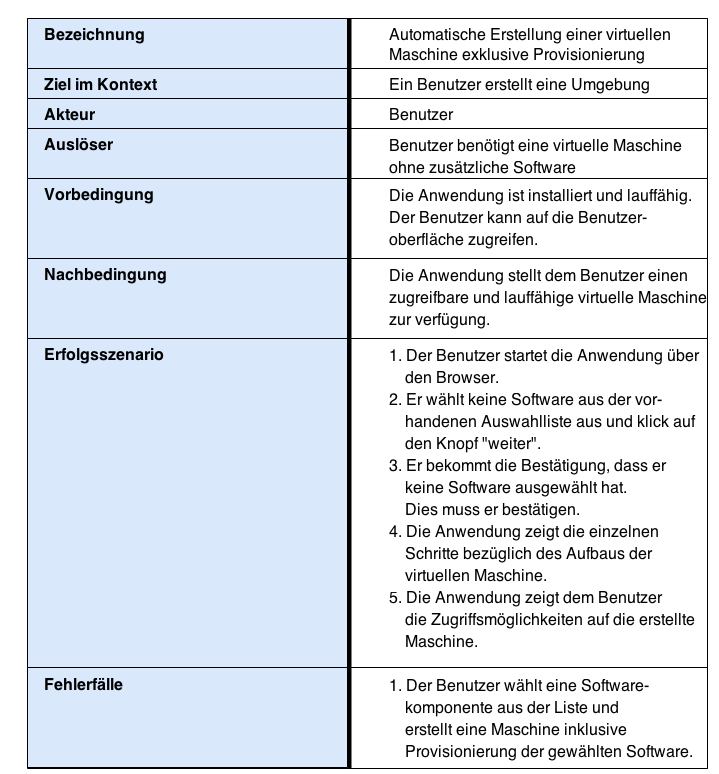
\includegraphics[scale=0.4]{../Bilder/usecase1.png}
\caption{Anwendungsfall AF 1}
\label{fig: dasdasdasdas}
\end{figure}

Anforderungen: [12312312312312312312]

\end{enumerate}
\setcounter{secnumdepth}{3}
\chapter{Die Software}
Dieses Kaptitel beschreibt die Entwicklung der Software, Designentscheidungen und die verwendeten externen Komponenten.

\section{Frontend}

\section{Backend}

\section{Ruby}
F�r die Entwicklung der Software wurde Ruby in der Version 1.9 im Zusammenhang mit dem Micro-Framework Sinatra verwendet.
Durch die leicht zu erlernenden Syntax und die einfache Wartung des Quellcodes, ist Ruby eine einsteigerfreundliche Programmiersprache, im Bereich der Webentwicklung.\newline 
Durch die Installation von Bundler, ein Dependency Manager f�r Ruby, werden alle ben�tigten Abh�ngigkeiten bei der Installation der hier thematisierten Software, heruntergeladen und installiert.
Somit entsteht ein zentraler Punkt, der sich um die Abh�ngigkeiten von Ruby k�mmert und es erm�glicht leicht und schnell �nderungen vorzunehmen.


\section{Externe Komponenten}
Die folgende Aufz�hlung gibt einen �berblick �ber die verwendeten Softwarekomponenten.\newline
Im nachfolgenden wird detaillierter auf die einzelnen Bauteile eingegangen und deren Funktionsweise ausf�hrlicher erkl�rt.
\begin{itemize}
      \item Sinatra
      \item Passenger      
	  \item Apache	  
	  \item SQLite      
      \item Vagrant
      \item VirtualBox
      \item Ansible
      \end{itemize}


\subsection{Sinatra}
Um die 


\subsection{Vagrant}
Vagrant  erm�glicht es durch wenig Aufwand eine schnell verf�gbare Umgebung aufzubauen.
Diese Arbeit bezieht sich in der Entwicklungsphase ausschlie�lich auf eine Ubuntu 32Bit Version, die Online von Vagrant bereitgestellt wird.
So wird eine stabile Testbasis erzeugt, die vom Hersteller gepr�ft wurde.\newline
Da Vagrant auf den g�ngigen Systemen OS X, Windows und diversen Linux Distrubutionen installiert werden kann, es hervorragend mit diversen Provisionierern zusammenarbeitet und VM-Tools wie VirtualBox, VMWare und AWS unterst�tzt, wird es zu einem guten Allrounder. \newline
Gerade die Provisionierung von Software, auf die zu startende virtuelle Maschine, macht Vagrant f�r das vorliegende Projekt attraktiv.
Zwar dauert der Aufbau im Gegensatz zu Docker nicht Sekunden sondern Minuten, aber die Provisionierung ist mit einer der entscheidende Punkte f�r die angestrebte Software.\newline
Die leicht zu handhabende Konfiguration und die eing�ngigen Begrifflichkeiten sind weiterer Punkte, die positiv f�r die Benutzung in diesem Projekt sprechen.


\subsection{Ansible}
 Ansible.......
%Quelle: Buch: ansible-for-devops

\section{Struktur und Zusammenspiel}
\section{Konfiguration}
\section{Datenbank}
Im Backend der Applikation befindet sich eine relationale Datenbank. \newline
Die dazu verwendete ORM-Schicht namens Datamapper unterst�tzt MySQL, PostgreSQL und SQLite.\newline
F�r den Prototypen der Anwendung wurde eine SQLite Datenbank benutzt um die Portierung auf andere Systeme zu erleichtern und den Installations-, sowie administrativen Aufwand gering zu halten.\newline
Allerdings ist SQLite weniger f�r Mehrbenutzerzugriffe ausgelegt, sondern f�r portable- und einbenutzer Anwendungen. Daher sollte die Datenbank in der Endfassung auf MySQL ge�ndert werden.\newline
Durch die verwendete ORM-Schicht, ist ein Austausch der Datenbank im Aufwand minimal.\newline
Die Datenbank beinhaltet die Softwarekomponenten, die zur Provisionierung der virtuellen Maschine eingesetzt werden k�nnen.
...

\section{Virtualisierung}
%Bild: http://www.digitalforreallife.com/wp-content/uploads/2012/11/django.png
\section{Provisionierung}
\section{Kommunikation der einzelnen Komponenten}
\section{Export Funktionen}

\subsection{Clonen einer Maschine}
Vagrant enth�lt nativ einen Befehlssatz, um aus einer aktuell laufenden Maschine eine wiederverwendbare Vagrant-Box zu erstellen.\newline
Um diese Box sp�ter wieder benutzen zu k�nnen, muss diese auf ein Laufwerk kopiert werden, welches von dem gew�nschten Mitarbeiter zugegriffen werden kann. Durch das Kopieren auf dessen lokalen Datentr�ger und dem Erstellen eines angepassten Import-Vagrantfiles, ist es m�glich Maschinen an Mitarbeiter weiterzugeben.
%Quelle: http://www.dev-metal.com/copy-duplicate-vagrant-box/

\subsection{Export zu Git}
Die Vorraussetzung hierf�r ist ein GitHub Konto, welches mit der Anwendung verkn�pft ist. \newline
Durch die Benutzung von GitHub, kann das zuvor erstellte Vagrantfile automatisiert als Git-Repository hochgeladen werden.\newline
Dies erm�glicht es Konfigurationen mit Mitarbeitern auszutauschen, zu archivieren oder zu versionieren.


\section{Sharing einer Maschine}
Mit der Version 1.5 hat Vagrant die M�glichkeit implementiert, eine erstellte Maschine mit anderen Mitarbeitern zu teilen.\newline
Da der Mitbenutzer nicht im gleichen Netzwerk sein muss, sondern einfach nur an das Internet angeschlossen sein braucht, ist diese Option...



\chapter{Grundlagen}
\chapter{Grundlagen}
Dieses Kapitel gibt einen Einblick in die verwendeten Programme, die f�r das Verst�ndnis der vorliegenden Arbeit von Vorteil sein k�nnen.
Es wird zun�chst auf die pr�gnanten Eigenschaften der Produkte eingegangen und wenn m�glich ein Vergleich mit Konkurrenzprodukten herangezogen.
Zudem wird teilweise die Handhabung und die Konfiguration kurz erl�utert.

\section{Ruby}
Die Programmiersprache Ruby wurde in etwa Mitte der 90er Jahre entwickelt und ist eine objektorientierte, dynamisch typisierte Sprache.
Sie zeichnet sich unter anderem durch ihre einfache und leicht erlernbare Syntax aus und ihrer einfachen Wartung des Quellcodes.
Bekannt geworden ist sie durch besonders durch das Framwork Ruby on Rails.\newline
Ruby Unterst�tzt diverse Programmierparadigmen, wie unter anderem prozedurale und funktionale Programmierung sowie Nebenl�ufigkeit und wird direkt von einem Interpreter verarbeitet. Au�erdem bietet die Sprache eine automatische Garbage Collection, Regul�re Ausdr�cke, Exceptions, Bl�cke als Parameter f�r Iteratoren und Methoden, Erweiterung von Klassen zur Laufzeit und Threads.\newline 
Da Ruby nicht Typisiert ist, wird alles als ein Objekt angesehen. Auf primitive Datentypen wird g�nzlich verzichtet.
%Quelle: http://b-simple.de/download/ruby.pdf
%Quelle: http://openbook.rheinwerk-verlag.de/it_handbuch/09_004.htm

\section{Sinatra} 
\section{Vagrant}
Bei Vagrant handelt es sich um ein Softwareprojekt, welches 2010 von Mitchell Hashimoto und John Bender 2010 ins Leben gerufen wurde.
Der prim�re Gedanke hinter diesem Projekt ist es, gerade Entwicklern und Teams eine schnelle und unkomplizierte M�glichkeit zu bieten, virtuelle Maschinen und Landschaften zu erstellen.\newline
%Vagrant ist also ein m�chtiges Werkzeug zum virtualisieren, der sonst oft lokalen Entwicklungsumgebungen. 
%Gerade Teamarbeit wird dadurch vereinfacht, denn die gew�nschten Maschinen k�nnen mit den gleichen Konfigurationen, Komponenten, Infrastrukturen und Bibliotheken erstellt werden.\newline 
Standardm��ig greift Vagrant auf VirtualBox zur�ck, um die Virtualisierung vorzunehmen. 
VirtualBox ist Oracles Freeware Pendant zur kommerziellen VMware Workstation/Fusion. Die Installation von Plugins erm�glicht es, statt auf VirtualBox auf VMware Workstation/Fusion oder Amazon Web Services zur�ckgegriffen werden.\newline 
Die Konfiguration einer Maschine geschieht �ber das 'Vagrantfile', in dem Parameter wie IP Adresse konfiguriert oder Provisionierer hinzuschaltet werden k�nnen. Bei den Provisionierern wird dem Benutzer die Freiheit gegeben, auf Bekannte wie Chef, Puppet oder Ansible zur�ckzugreifen.\newline
Da das Vagrantfile in einer Ruby Domain Specific Language geschrieben wird, bedeutet das f�r den Anwender, dass er es einfach mit anderen Kollegen �ber Versionskontrollen (z.B. Git oder Subversion) teilen kann.\newline
Abgesehen von dem Austausch der Konfigurationen, wird die Teamarbeit durch eine 'sharing' Option unterst�tzt, die mit Version 1.5 implementiert wurde.
Das Teilen eine Maschine erm�glicht es Teams an gemeinsamen und entfernten Standorten auf die gleiche Maschine zuzugreifen. 

\subsection{Konfiguration}
Vagrantfile beinhalten die Konfiguration jeder Vagrantmaschine. Sogar jeder Vagrant-"Landschaft". 
Das in Ruby Syntax geschriebene Konfigurationsfile, wird automatisch �ber den Befehl 'vagrant init' im gew�nschten Ordner generiert oder manuell �ber jeden Editor erstellt werden. Auf Linux-Systemen ist darauf zu achten, dass der gew�nschte Ordner �ber entsprechende Berechtigungen verf�gt.
Manuelle Erweiterung des Vagrantfiles wird durch die Rubysyntax zus�tzlich vereinfacht.


\subsection{Vergleich zu Docker}
%Im Zusammenhang mit ad hoc Umgebungen, liegt der Fokus in Diskussion oft auf Docker und Vagrant.
%Der Grundgedanke bei beiden Applikationen ist der Gleiche, aber man muss sich bewusst sein, was das Ziel der Anwendung sein soll.
%Beide Applikationen haben wie alles ihre Vor- und Nachteile, aber in einem sind beide Virtualisierungs-Tools gleich. Die zentrale Steuerung zum Aufbau einer %Maschine, geschieht �ber ein einziges Konfig-File.\newline
Docker ist ein Linux-only VE (Virtual Environment)-Tool und arbeitet im Gegensatz zu Vagrant mit Operating-System-Level Virtualisierung, auch Linux Containern (LxC) genannt. W�hrend Vagrant Hypervisor-basierten virtuellen Maschinen aufbaut.
F�r die sogenannten Container nutzt Docker spezielle Kernelfunktionalit�ten, um einzelne Prozesse in Containern voneinander zu isolieren.\newline 
Dadurch wird f�r den Benutzer der Eindruck erweckt, dass f�r Prozesse die mit Containern gestartet werden, diese auf ihrem eigenen System laufen w�rden.
Docker wird in drei Teile unterteilt. Die Arbeitsweise ist nicht wie bei einer VM (virtuelle machine) bei der ein virtueller Computer mit einem bestimmten Betriebssystem, Hardware-Emulation sowie Prozessor simuliert wird. Ein VE ist quasi eine leichtgewichtige virtuelle Maschine. In einem Container ausgef�hrte Prozesse greifen gemeinschaftlich auf den Kernel des Hostsystems zu. Durch die Kernelnamensr�ume(cnames) werden die ausgef�hrten Prozesse voneinander isoliert. Allerdings ist gerade die Isolation der Prozesse, durch den gemeinsam genutzten Kernel etwas geringer, als bei der Benutzung durch einen Hypervisor.\newline
Durch die zugrunde liegende Architektur von Vagrant, wird Vagrant gerne f�r immer gleich aufbauende Entwicklungsumgebungen benutzt.
Die Vielzahl an unterst�tzten Betriebssystemen macht es f�r viele Benutzer attraktiver. Allerdings kooperieren Vagrant und Docker auch hervorragend zusammen.
%Vagrant verspricht durch die leichtere Handhabung und Konfiguration eher das, was f�r das vorliegende Projekt entscheidend ist.



%ZITAT: Docker wird in diversen Varianten als L�sung f�r das Setup und die Kapselung lokaler Entwicklungsumgebungen, als tempor�r verf�gbarer Service imRahmen von Integrationstests und als Laufzeitumgebung auf Produktionsservern eingesetzt. Gerade der tempor�re Charakter von Docker-Containern wird f�r einen anderen Anwendungsfall interessant: als dynamisch erzeugte Buildsysteme mit einer projektspezifischen Buildumgebung.
%Quelle: http://www.scriptrock.com/articles/docker-vs-vagrant 
%Quelle: https://entwickler.de/online/docker-basics-system-level-virtualisierung-125514.html







\section{Ansible}

\subsection{Vergleich zu Salt}
Da Ansible mit Salt am ehesten verwandt ist, wird auf Puppet und Chef im weiteren nicht weiter eingegangen.
Puppet und Chef wiedersprechen dem vorgesehenen Konzept der leichten Konfiguration.

Salt ist wie Ansible in Python entwickelt worden. Da Salt zur Kommunikation mit seinen Clients Agenten (Minions) ben"otigt, ist dies wiederrum schwer zu automatisieren. Zwar kann Vagrant mit Salt zusammenarbeiten, allerdings nicht nativ. Salt w"are eine gute Alternative, wenn nicht nur einen Provisioner haben m"ochte, sondern auch ein remote execution framework.
Salt implementiert eine ZeroMQ messaging lib in der Transportschicht, was die Kommunikation zwischen Master und Minions im Gegensatz zu Chef und Puppet vervielfacht. Dadurch ist die Kommunikation zwar schnell, aber nicht so sicher, wie bei der SSH Kommunikation von Ansible. 
ZeroMq bietet keine native Verschl"usselung und transportiert Nachichten "uber IPC, TCP, TIPC und Multicast.

http://www.scriptrock.com/articles/ansible-vs-salt

\subsection{Vergleich zu Puppet}
Einer der wohl bekanntesten Configuration Management Tool ist Puppet.
Puppet wird von allen g"angigen Betriebssystemen unterst"utzt. Windows, Unix, Mac OS X und Linux. 

Nachteile: Flexibilit"at und Agilit"at sind keine st"arken. Zu gro{/ss}. 

\include{sinatra}
\section{Passenger}
\section{Sidekiq}
\chapter{Schluss}
\section{ Zusammenfassung}
\section{Fazit}
%%%%
%% add some text to generate a sample document
%%%\setcounter{secnumdepth}{3}
\chapter{Einleitung}
\begin{quote}
	``Es ist nicht zu wenig Zeit, die wir haben, sondern es ist zu viel Zeit, die wir nicht nutzen'' - Lucius Annaeus Seneca, \cite{Apelt200511}
\end{quote}
Seneca formulierte  49 n. Chr. ein Gef"uhl das jeder kennt. Die Zeit die er hat, nicht richtig zu nutzen.
Technische Neuerungen helfen uns unsere Zeit besser zu planen, mehr Zeit in andere Aktivit�ten zu stecken und unsere Priorit�ten zu "uberdenken.
Diese Arbeit besch�ftigt sich mit dem Teil-Aspekt der Informatik, der Virtualisierung von Servern im Entwicklungsumfeld.\newline
... 


\section{Motivation}
\textbf{TODO}
[...]
Die Motivation dieser Ausarbeitung besteht darin, eine Software zu entwickeln, die durch vereinfachte Handhabung und minimaler Einarbeitungszeit, es dem Benutzer erm�glich eine ad-hoc Umgebung zu erstellen, ohne b�rokratischen Aufwand und ohne Grundwissen �ber die darunterliegende Anwendungsstruktur.
Der normalerweise gro�e zeitliche Aufwand soll m�glichst minimiert werden und es Anwendern in Unternehmen und Projekten erleichtern, sich auf die vorhandenen Usecase zu fokussieren und keine Zeit in Aufbau, Installation und Problembehebung investieren zu m�ssen. [...]

\section{Zielsetzung}
Das Ziel der vorliegenden Arbeit ist es, durch inkrementelles und interatives Vorgehen eine Applikation zu modellieren, die den Anwender der Applikation bei dem Aufbau von virtuellen Umgebungen unterst�tzt. Je nach Wunsch des Anwenders, wird nicht nur der Aufbau einer Umgebung vereinfacht, sondern auch die direkte Installation von Programmen veranlasst. Eine Weboberfl�che soll die entsprechenden Optionen zur Verf�gung stellen und dem Anwender durch seine ausgew�hlte Funktion leiten.
Gro�e Konfigurationen oder komplizierte Einstellungen sollen dem Normalanwender abgenommen werden und geschehen im Hintergrund. 
Damit auch ein Sichern oder ein Zur�ckspielen von vorhandenen virtuellen Maschinen m�glich wird, sollten Im- und Exportfunktionen dies untzerst�tzen.
Die Realisierung sollte auf einem zentralen Knotenpunkt stattfinden, um es mehreren Anwendern zu erm�glichen, ihre notwendige Maschine zu erstellen und zu verwalten.
Kernaufgaben sollen Open-Source Anwendungen �bernehmen, die in ihrem Bereich etabliert sind. Ebenfalls im Fokus steht die Leichtigkeit der Konfiguration der auszuw�hlenden Open-Source Anwendung.
Bei der Erstellung der einzelnen Softwarekomponenten ist stehts auf das Prinzip von hoher Koh�sion und loser Kopplung zu achten. Also dem Grad der Abh�ngigkeit zwischen mehrere Hard-/ und Softwarekomponenten, der �nderungen an einzelnen Komponenten erleichtert.
Um auch die Anwendungsoberfl�che unkompliziert zu halten, soll der Anwender mit ein paar Klicks zu seinem Ziel gef�hrt werden. Durch das Vermeiden von unn�tigen Verschachtelungen oder einer Flut an Optionen und Konfigurationen, soll der Anwender in der Applikation einen Helfer f�r seine T�tigkeit finden.
\newline


\begin{comment}


\section{Problemstellung}
%Die Einleitung muss Ihr Thema eingrenzen (und diese Eingrenzung rechtfertigen) und Ihr Erkenntnisinteresse präzisieren und begründen
Virtualisierung hat in vielen Bereichen den physischen Server abgel�st, denn der Finanzielle Aspekt ist f"ur Unternehmen nicht unerheblich. Im Idealfall hei�t der Umstieg auf virtuelle Landschaften gleich weniger Server, was gleichbedeutend mit weniger Stellfl�che ist. Somit auch mit weniger Racks und weniger Verkabelung.\newline
Aufw�ndige Vorplanung von Serverzentren entf�llt, die Kostenplanung der unterschiedlichen Hardware wird minimiert und die Frage, was in ein paar Jahren mit der Hardware passieren soll, wird obsolet.\newline
Gerade im Entwicklungsbereich ist es meist sinnvoller virtuelle Umgebungen zu realisieren, als reale Maschinen aufzubauen. Entwickler haben so die M�glichkeit bei Bedarf sich Abz"uge der Produktionsumgebung zu erstellen oder Fehlerszenarien nachzustellen.\newline
Meist ist dazu die Involvierung des Betriebs-Teams oder des IT-Support notwendig, die nach Priorit�t ihrer Auftragslage, eine gewissen Vorlaufzeit ben�tigen, um die gew�nschte Maschine aufzubauen. \newline
In dem Fall, dass die Firmengr��e es nicht erlaubt, eine eigene Support-Abteilung zu haben, muss die Zeit des jeweiligen Mitarbeiters herhalten, um das Wissen �ber die jeweilige Virtualisierungsl�sung aufzubauen, die gew�nschte Maschine zu erstellen und die Installationen der n�tigen Programme zu realisieren. Der R�ckschluss daraus ist, geringere Produktivit�t in den Kernt�tigkeiten des Mitarbeiters.\newline
Auch wenn die Softwarebranche eine Vielfalt an M�glichkeiten bereitstellt, sind diese entweder in ihrer Struktur �berdimensioniert, um sie in der Anwendung schnell zu erlernen, oder komplex in ihrer Konfiguration in Bezug auf Automatisierungen und/oder Provisionierungen.

\end{comment}

\section{Themenabgrenzung}
Diese Arbeit greift bekannte und etablierte Softwareprodukte auf und nutzt diese in einem zusammenh�ngenden Kontext. Dabei werden die verwendeten Softwareprodukte nicht modifiziert, sondern f�r eine vereinfachte Benutzung durch eigene Implementierungen kombiniert und mit einem Benutzerinterface versehen, welches die Abl�ufe visualisiert und dem Benutzer die Handhabung vereinfacht.
Die vorzunehmenden Implementierungen greifen nicht in den Ablauf der jeweiligen Software ein, sondern vereinfacht das Zusammenspiel der einzelnen Anwendungen.



\section{Struktur der Arbeit}
[...]

\chapter{Grundlagen}
[...]
%Dieses Kapitel gibt einen Einblick in die Grundlagen der Virtualisierung.
%Dieses Kapitel soll die Einblick in die Grundlagen der Virtualisierung geben.
%Zun�chst wird erl�utert, was Virtualisierung ist, dann werden Begrifflichkeiten gekl�rt sowie Vor- und Nachteile begutachtet.

\section{Grundlagen der Virtualisierung}
F�r den Begriff Virtualisierung existiert keine allgemeing�ltige Definition. In der Regel wird damit der parallele Einsatz mehrerer Betriebssysteme beschrieben oder detailierter, das Ressourcen zu einer logischen Schicht zusammengefasst werden und dadurch deren Auslastung optimiert wird. So kann die logische Schicht bei Aufforderung ihre Ressourcen automatisch zur Verf�gung stellen. 
Das Prinzip dahinter ist die Verkn�pfung von Servern, Speichern und Netzen zu einem virtuellen Gesamtsystem.
Daraus k�nnen sich dar�ber liegende Anwendungen direkt und bedarfsgerecht ihre Ressourcen beziehen.\newline
Grunds�tzlich unterscheidet man zwischen 
\begin{enumerate}
\item \textbf{Virtualisierung von Hardware}\newline
die sich mit der Verwaltung von Hardware-Ressourcen besch�ftigt und
\item \textbf{Virtualisierung von Software}\newline 
die sich mit der Verwaltung von Software-Ressourcen, wie z.B. Anwendungen und Betriebssystemen besch�ftigt.
\end{enumerate}
[\cite{Bengel200806}]



\subsection{Virtuelle Maschine}\label{subsec:VirtuelleMaschine}
Eine virtuelle Maschine ist nach Robert P. Goldberg
\begin{quote}
\textit{'a hardware-software duplicate of a real existing computer system in
which a statistically dominant subset of the virtual processor's
instructions execute directly on the host processor in native mode'} [\cite{SiegertBaumgarten200612}]
\end{quote} 
W�rtlich �bersetzt ist also eine virtuelle Maschine ein Hardware-/Software-Duplikat eines real existierenden Computersystems, in dem eine statistisch dominante Untermenge an virtuellen Prozessoren, Befehle im Benutzer-Modus auf dem Host-Prozessor ausf�hren.
Dieses Duplikat kann als Software-Container betrachtet werden, der einen vollst�ndigen Satz an emulierten Hardwareressourcen, dem Gastbetriebssystem und entsprechenden Anwendungen besteht. Durch die Containerstruktur wird eine Kapselung hervorgerufen, die es erm�glicht mehrere virtuelle Maschinen komplett unabh�ngig auf einem Hostsystem zu installieren und laufen zu lassen. Ist eine virtuelle Maschine fehlerhaft oder nicht mehr erreichbar, betrifft dies nicht automatisch die restlichen parallel laufenden Maschinen und stellt damit einen der charakteristischen Vorteile von virtuellen Maschinen dar. Die Verf�gbarkeit. Backup-Systeme oder mehrere Instanzen einer Applikationen k�nnen so unabh�ngig auf einem Host ausgef�hrt werden, ohne sich gegegnseitig zu beeinflussen. Durch den struktuellen Aufbau einer virtuellen Maschine, ist es ebenfalls m�glich, eine Maschine nach den eigenen W�nschen zu erstellen und diese im Weiteren zu replizieren.\newline
Virtuelle Maschinen k�nnen ohne gr��eren Aufwand verschoben, kopiert und zwischen Hostservern neu zugeteilt werden, um die Hardware-Ressourcen-Auslastung zu optimieren. Administratoren k�nnen auch die Vorteile von virtuellen Umgebungen f�r einfache Backups, Disaster Recovery, neue Deployments und grundlegenden Aufgaben der Systemadministration nutzen, da das Wiederherstellen aus Speicherpunkten oder gespeicherten Abz�gen, innerhalbt von Minuten zu realisieren ist.\newline


\subsection{Gastbetriebssystem}\label{subsec:Gastbetriebssystem}
Ein �bliches Betriebssystem wird im privilegierten Prozessor-Modus ausgef�hrt (Auch Kernel-Mode genannt). Dies bef�higt es, die absolute Kontrolle �ber die vorhandenen Ressourcen zu gewinnen. Alle Anwendungen, die auf dem Betriebssystem laufen, werden im sogenannten Benutzer-Modus ausgef�hrt. Die Privilegien im Benutzer-Modus sind allerdings relativ eingeschr�nkt. Ein direkter Zugriff wird nur sehr selten und unter genau kontrollierten Bedingungen gestattet. Dies hat den Vorteil, dass kein Programm z. B. durch einen Fehler das System zum Absturz bringen kann. (\cite{Reuther2014})\newline
Eine virtuelle Maschine (siehe \ref{subsec:VirtuelleMaschine}) l�uft als normaler Benutzer-Prozess im Benutzer-Modus, was zur Folge hat, dass das dort installierte Betriebssystem, das Gastbetriebssystem, folglich nicht den privilegierten Prozessor-Modus nutzen kann, wie es ein nicht virtualisiertes Betriebssystem k�nnte. Da weder die Anwendungen noch das entsprechende Gastbetriebssystem Kentniss dadr�ber haben, dass sie in einer virtuellen Maschine laufen, m�ssen ausgef�hrte Instruktionen, die den Prozessor-Modus erfordern, entsprechend anders gehandhabt werden. Dies ist unter anderem die Aufgabe des Hypervisors (siehe \ref{subsec:Hypervisor}).


\begin{center}
 \begin{minipage}{\linewidth}
	\centering
	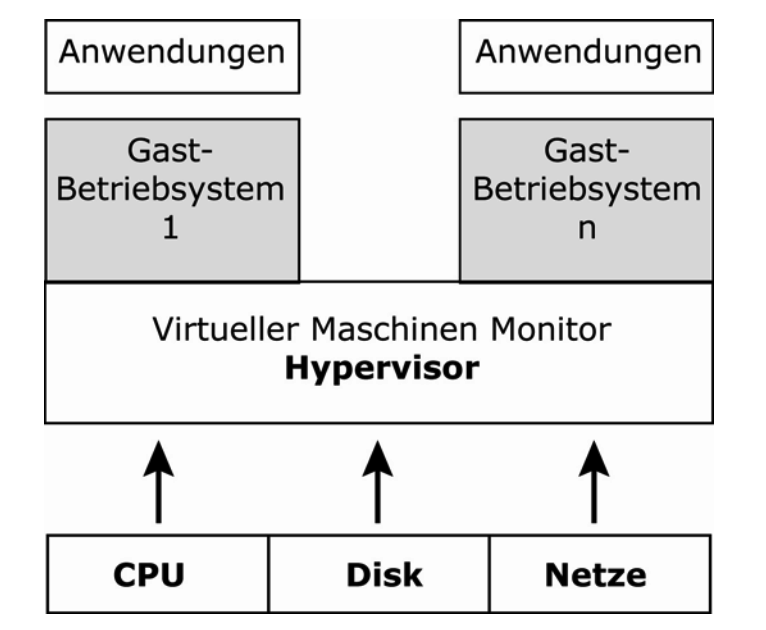
\includegraphics[scale=0.4]{../Bilder/BSVirtualisierung.png}%
	\captionof{figure}[Betriebssystemvirtualisierung]{Betriebssystemvirtualisierung [\cite{SiegertBaumgarten200612}]}%
	\label{fig:Betriebssystemvirtualisierung}% 
 \end{minipage}
\end{center}


\subsection{Hypervisor}\label{subsec:Hypervisor}
Der Name des Hypervisors kann von Hersteller zu Hersteller variieren. Bei Microsoft z.B.  wird er Hyper-V genannt und bei VMware als ESXi bezeichnet.
Der Hypervisor, oder in der Literatur auch VMM (Virtual Machine Monitor) genannt, ist die sogenannte abstrahierende Schicht zwischen der tats�chlich vorhanden Hardware und den ggf. mehrfach existierenden Betriebssystemen. Siehe \ref{fig:Betriebssystemvirtualisierung}.
Seine prim�re Aufgabe ist die Verwaltung der Host-Ressourcen und deren Zuteilung bei Anfragen der Gastsysteme. L�sen Instruktionen, oder Anfagen eines Gastbetriebssystems eine CPU-Exception aus, weil diese im Benutzer-Modus ausgef�hrt werden, f�ngt der Hypervisor diese auf und emmuliert die Ausf�hrung der Instruktionen (trap and emulate). Die Ressourcen des Hostsystems werden derart verwaltet, dass diese bedarfsgerecht zur Verf�gung stehen, egal ob ein oder mehrere Gastsysteme laufen. Zudem z�hlt unter anderem E/A-Zugriffe (insbesondere Hardwarezugriffe), Speichermanagement, Prozesswechsel und System-Aufrufe.\newline
Den Hypervisor kann man in zwei verschiedene Typen kategorisiert.
\begin{description}
\item  [Typ 1 Hypervisor]\hfill \\
arbeitet direkt auf der Hardware und ben�tigt somit kein Betriebssystem, welches zwischen ihm und der Hardware liegt. Alle dar�ber liegenden virtuelle Maschinen laufen in sogenannten Domains. Weder der Hypervisor noch die anderen Domains sind f�r die jeweilige Domain sichtbar. Die Verwaltung der laufenden Domains wird durch eine priviligierte Domain geregelt, die in der Dom0 l�uft. Dadurch hat die priviligierte Domain die M�glichkeit andere Domains zu starten, stoppen und zu verwalten. \newline
Der Hypervisor Type-1 verf�gt selbst �ber die n�tigen Ger�tetreiber, um den virtuellen Maschinen CPU, Speicher und I/O zur Verf�gung zu stellen. Durch die wegfallende Schicht, das nicht ben�tigte Betriebssystem, gewinnt der Hypervisor Typ 1 an Performance und spart am Ressourcenverbrauch. Siehe Abbildung [\ref{fig:KlassifizierungHypervisor}.a].

\item  [Typ 2 Hypervisor]\hfill \\
l�sst durch seine Bezeichnung als 'Hosted' erahnen, dass der Unterschied zu Typ 1 darin besteht, dass er auf einem Hostsystem aufsetzt. Also eine Schicht implementiert sein muss, die zwischen dem Hypervisor und der Hardware liegt. Siehe Abbildung [\ref{fig:KlassifizierungHypervisor}.b].\newline
Diese Schicht wird durch ein Betriebssystem realisiert, das dem Hypervisor den Zugang zur Hardware durch die eigenen Hardwaretreiber erm�glicht.
Ist ein Betriebssystem mit einer Hardware kompatibel, ist transitiv gesehen, der Hypervisor ebenfalls mit installier- und ausf�hrbar. Dies vereinfacht die Installation gegen�ber dem Hypervisor Typ 1. \newline
Aus Implementierungssicht gibt es f�r beide Hypervisoren Vor- und Nachteile.
F�r einige Bereiche ist die Anforderung eines Betriebssystems nur von Vorteil.
Vor allem wenn es um um Hardware- und Treiber-Kompatibilit�t, Konfigurationsflexibilit�t und vertraute Management-Tools geht.\newline
Auf der anderen Seite kann genau das zum Nachteil ausgelegt werden.
Es entsteht nicht nur ein h�herer Management-Aufwand um das Betriebssystem zu konfigurieren und zu verwalten, auch die Performance und der Sicherheitsaspekt leiden unter dieser zus�tzlichen Schicht. 
\end{description}
\begin{figure} 
    \subfigure[Bezeichnung der linken Grafik]{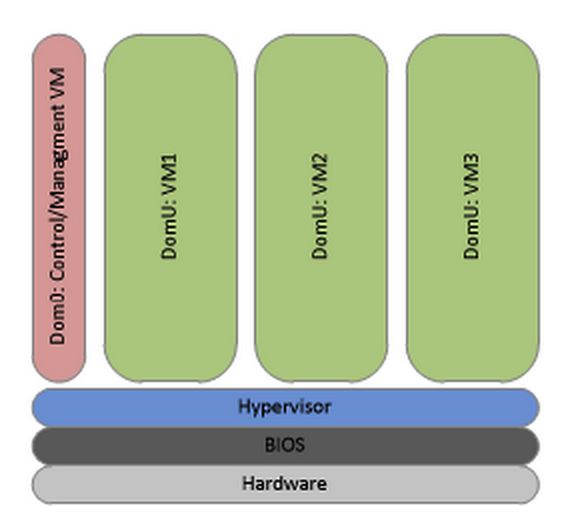
\includegraphics[width=0.49\textwidth]{../Bilder/Hypervisor1.png}} 
    \subfigure[Bezeichnung der rechten Grafik]{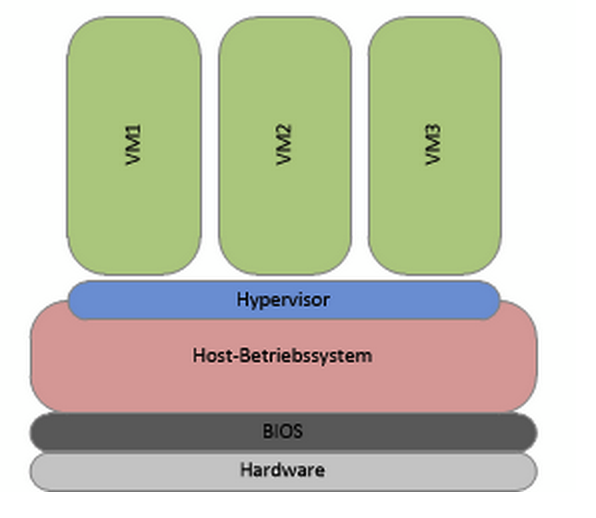
\includegraphics[width=0.49\textwidth]{../Bilder/Hypervisor2.png}} 
\label{fig:KlassifizierungHypervisor}%
\caption{Hypervisor Typ 1 und 2} 
\end{figure} 

\section{Provisioning/Konfigurationsmanagement}\label{subsec:Provisioning}
\textbf{TODO: WELCHER BEGRIFF IST BESSER?}\newline
Die Hauptaufgabe eines Konfigurationsmanagement-Systems, im folgenden nur noch KMS genannt, ist es, eine zuvor definierte Zustandsbeschreibung eines Hosts umzusetzen. Dies kann das Installieren von Softwarepaketen bedeuten, starten oder beenden von Diensten oder  Konfigurationen erstellen/anpassen/entfernen zu lassen.
In der Regel verwenden KMS eigene Agenten auf den Zielsystemen, �ber die die Kommunikation l�uft und die Zustandsbeschreibung realisiert wird. Neuere Anwendungen wie 'Ansible' aus Kapitel \ref{subsec:Ansible}, die Konfigurationsmanagement unterst�tzen, ben�tigen diese Agenten nicht mehr und realisieren die Kommunikation �ber eine SSH-Schnittstelle.
Pull-basierte Tools, wie beispielsweise 'Puppet', fragen in regelm�ssigen Abst�nden ein zentrales Konfigurations-Repository ab, in dem die jeweils aktuelle Zustandsbeschreibung der Maschine gespeichert ist und sorgt daf�r, dass die �nderungen auf dem Client ausgef�hrt werden.
Es spielt keine Rolle, ob der Zielclient eine virtuelle Maschine ist oder eine standard Maschine ist. KMS sind in der Regel dazu f�hig ganze Gruppen an Rechner parallel zu bearbeiten und die entsprechenden Zustandsbeschreibungen umzusetzen. 
Bei dem im oberen Abschnitts bereits genannten Beispiel 'Ansible', k�nnen mehrere Rechner simpel in Inventory-Dateien als Gruppen zusammengefasst werden, die dann jeweils durch 'Ansible' angesprochen werden k�nnen um entsprechende St�nde an Zustandsbeschreibungen dort auszuliefern. Siehe \ref{lst:InventoryDatei}

\begin{lstlisting} [caption={Beispiel Inventory-Datei}\label{lst:InventoryDatei},captionpos=t] 
[atomic]
 192.168.100.100
 192.168.100.101
[webserver]
 192.168.1.110
 192.168.1.111
 \end{lstlisting}

%Quelle: http://www.admin-magazin.de/Online-Artikel/Konfigurationsmanagement-mit-Ansible
\begin{comment}
\section{Begriffserkl�rung}
Im Verlauf dieser Arbeit werden Begrifflichkeiten verwendet, die im Vorfeld zu kl�ren sind.\newline
	\begin{enumerate}
		\item \textbf{Provisioning / Provisioner}\newline
\textit{Provisioning} ist ein Aspekt der Informatik, in dem es darum geht, den richtigen Personen zur richtigen Zeit effektiv Ressourcen zur Verf�gung zu stellen.
\textit{Provisioner} helfen bei der Softwareverteilung auf gew�nschte Maschinen, Ad-hoc Kommando-Ausf�hrung und Konfigurationsmanagement.
In dieser Arbeit bezieht sich der Begriff \textit{Provisioning} auf die automatisierte Softwareverteilung, die mit dem Aufbau einer Entwicklungsumgebung verbunden ist.\newline
		\item \textbf{Entwicklungsumgebung}\newline
IDE's (integrated development environment) sind Entwicklungsumgebungen, die den Entwickler unterst�tzen, Quellcode zu schreiben und zu bearbeiten. Die g�ngigsten IDE's unterst�tzen meist mehrere Programmiersprachen und helfen dem Entwickler mit n�tzlichen Funktionen, wie  z.B. das aufzeigen von Fehlern im Quelltext. Entwicklungsumgebungen sind in vielen F�llen auch PC's / Server / virtuelle Maschinen, die zum Entwickeln installiert und bereitgestellt werden.
Dort k�nnen neue Funktionalit�ten ausprobiert werden und das bestehende System testweise erweitert werden, ohne in die Produktionslandschaft einzugreifen.
In den folgenden Texten wird der Begriff \textit{Entwicklungsumgebung} als Synonym f�r eine virtuelle Maschine benutzt, die dem Anwender die Freiheit gibt, unkompliziert M�glichkeiten auszutesten und neues auszuprobieren.\newline
		\item \textbf{Aufbau einer Maschine}\newline
\textit{Aufbau einer Maschine} beinhaltet immer das automatische Erstellen und Konfigurieren einer virtuellem Maschine mit Hilfe von VirtualBox und Vagrant.
Das Resultat ist eine virtuelle Maschine mit der Basisinstallation von Ubuntu (32Bit / 64Bit) und \textbf{MEHR INFOS ZU DEM SYSTEM}.
Durch die M�glichkeit des Provisioning kann die Basisinstallation mit Software erg�nzt und Befehle auf der Maschine ausgef�hrt werden.

\item \textbf{Maschinenkonfiguration}\newline
F�r den Aufbau einer Maschine werden zwei wesentliche Konfigurationsdateien erstellt.
Diese werden f�r den Aufbau der virtuelle Maschine selbst ben�tigt und f�r das ggf. gew�nschte Provisioning. Der Begriff \textit{Maschinenkonfiguration} beschreibt im folgenden immer das Vorhandensein beider Dateien. 
\end{enumerate}
\end{comment}


%%\subfile{Einleitung}



%\lipsum

See also \cite{goossens93}.
%%%%

%% appendix if used
%%\appendix
%%\typeout{===== File: appendix}
%%\include{appendix}

% bibliography and other stuff
\backmatter

\typeout{===== Section: literature}
%% read the documentation for customizing the style
\bibliographystyle{dinat}
\bibliography{literatur}

\typeout{===== Section: nomenclature}
%% uncomment if a TOC entry is needed
%%\addcontentsline{toc}{chapter}{Glossar}
\renewcommand{\nomname}{Glossar}
\clearpage
\markboth{\nomname}{\nomname} %% see nomencl doc, page 9, section 4.1
\printnomenclature

%% index
\typeout{===== Section: index}
\printindex

\HAWasurency

\end{document}
